\documentclass[border=10pt]{standalone}
\usepackage{tikz}
\usetikzlibrary{chains, positioning}
\begin{document}
    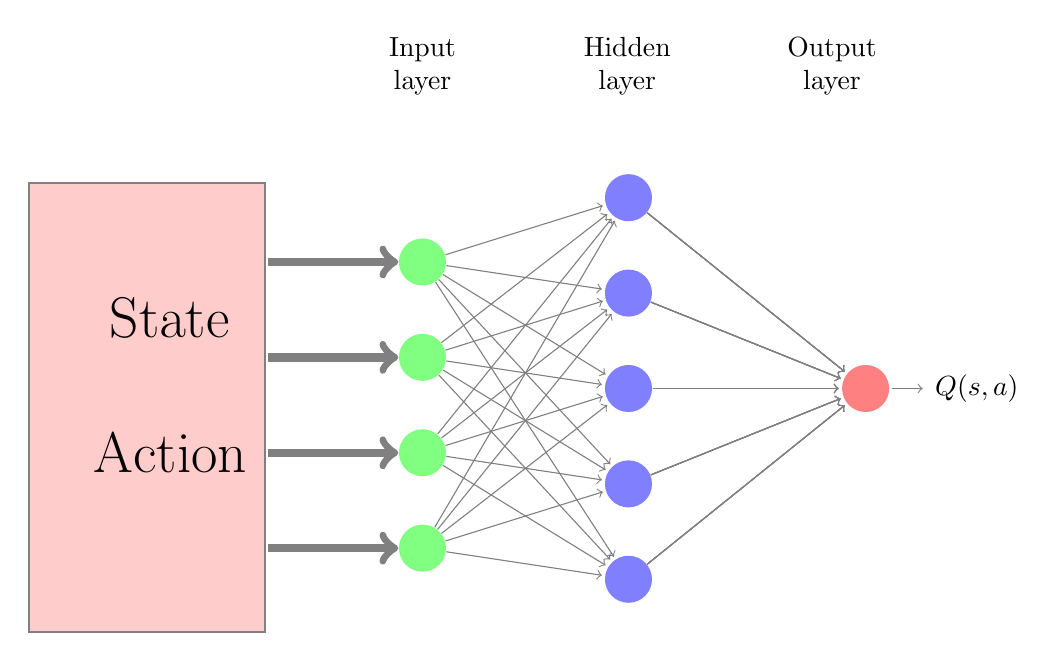
\begin{tikzpicture}[shorten >=1pt,
                    ->, draw=black!50, 
                    node distance = 6mm and 24mm,
                    start chain   = going below,
                    every pin edge/.style = {<-,shorten <=1pt},
                    neuron/.style = {circle, fill=#1, minimum size=17pt, 
                                     inner sep=0pt, on chain},
                    annot/.style = {text width=4em, align=center}]
    
        % code copied from the neural network digrams
        \foreach \i in {1,...,4}
            \node[neuron=green!50] (I-\i)    {}; 
        
        \node[neuron=blue!50, above right=6mm and 24mm of I-1.center] (H-1) {};
        
        \foreach \i [count=\j from 1] in {2,...,5} 
            \node[neuron=blue!50, below=of H-\j] (H-\i) {};
            
         \node[neuron=red!50,  pin={[pin edge=->]0: $Q(s, a)$}, right=of H-3]     (O-1) {};
         
        \foreach \i in {1,...,4}
            \foreach \j in {1,...,5}
            {
                \path (I-\i) edge (H-\j)
                      (H-\j) edge (O-1);
            }
            
        % code written after some understanding and google search (Final motive - try before googling)
        \foreach \i in {1, ..., 4}
            \path[draw, <-, line width=3pt] (I-\i) -- +(-2, 0);    
        
        \path[draw, fill=red!20, thick] (-5, 1) rectangle (-2, -4.7)                node[pos=0.3, right]  {\huge{State}} 
            node[pos=0.6] {\huge Action};

            
        \foreach \l [count=\x from 0] in {Input, Hidden, Output}
          \node [align=center, above] at (\x * 2.6, 2) {\l \\ layer};
        
    \end{tikzpicture}
\end{document}